%versi 2 (8-10-2016)
\chapter{Landasan Teori}
\label{chap:teori}

\section{Skripsi}
\label{sec:skripsi} 
 
Rencananya akan diisi dengan penjelasan umum mengenai buku skripsi.

\dtext{11-12} 

\section{\LaTeX}
\label{sec:latex}

Mengapa menggunakan \LaTeX{} untuk buku skripsi dan apa keunggulan/kerugiannya bagi mahasiswa dan pembuat template. 

\dtext{13-14}


\section{Template Skripsi FTIS UNPAR}
\label{sec:template}
 
Akan dipaparkan bagaimana menggunakan template ini, termasuk petunjuk singkat membuat referensi, gambar dan tabel.
Juga hal-hal lain yang belum terpikir sampai saat ini. 
 
\dtext{15-16}

\subsection{Tabel}  
Berikut adalah contoh pembuatan tabel. 
Penempatan tabel dan gambar secara umum diatur secara otomatis oleh \LaTeX{}, perhatikan contoh di file bab2.tex untuk melihat bagaimana cara memaksa tabel ditempatkan sesuai keinginan kita.

Perhatikan bawa berbeda dengan penempatan judul gambar gambar, keterangan tabel harus diletakkan di atas tabel!!
Lihat Tabel~\ref{tab:contoh1} berikut ini:

\begin{table}[H] %atau h saja untuk "kira kira di sini"
	\centering 
	\caption{Tabel contoh}
	\label{tab:contoh1}
	\begin{tabular}{cccc}
		\toprule
		& $v_{start}$ & $\mathcal{S}_{1}$ & $v_{end}$\\

		\midrule
		$\tau_{1}$ & 1 & 12& 20\\
		$\tau_{2}$ & 1 &  & 20\\
		$\tau_{3}$ & 1 & 9 & 20\\
		$\tau_{4}$ & 1 &  & 20\\

		\bottomrule
		
	\end{tabular} 
\end{table}
Tabel~\ref{tab:cthwarna1} dan Tabel~\ref{tab:cthwarna2} berikut ini adalah tabel dengan sel yang berwarna dan ada dua tabel yang bersebelahan. 
\begin{table}[H]
	\begin{minipage}[c]{0.49\linewidth}
		\centering
		\caption{Tabel bewarna(1)}
		\label{tab:cthwarna1}
		\begin{tabular}{ccccc}
			\toprule
			 & $v_{start}$ & $\mathcal{S}_{2}$ & $\mathcal{S}_{1}$ & $v_{end}$\\
			
			\midrule
			$\tau_{1}$ & 1 & 5 \cellcolor{green}& 12& 20\\
			$\tau_{2}$ & 1 & 8 \cellcolor{green}& & 20\\
			$\tau_{3}$ & 1 & 2/8/17 \cellcolor{green}& 9 & 20\\
			$\tau_{4}$ & 1 & \cellcolor{red}& & 20\\
			
			\bottomrule

		\end{tabular}
	\end{minipage}
	\begin{minipage}[c]{0.49\linewidth}
		
		\centering 
		\caption{Tabel bewarna(2)}
		\label{tab:cthwarna2}
		\begin{tabular}{ccccc}
			\toprule
			 & $v_{start}$ & $\mathcal{S}_{1}$ & $\mathcal{S}_{2}$ & $v_{end}$\\
			
			\midrule
			$\tau_{1}$ & 1 & 12& 5 \cellcolor{red} &20\\
			$\tau_{2}$ & 1 &  &  8 \cellcolor{green} &20\\
			$\tau_{3}$ & 1 & 9 & 2/8/17 \cellcolor{green} &20\\
			$\tau_{4}$ & 1 &   & \cellcolor{red} &20\\
			
			\bottomrule
		
		\end{tabular}
	\end{minipage}
\end{table}

 
\subsection{Kutipan}
\label{subs:kutipan} 
Berikut contoh kutipan dari berbagai sumber, untuk keterangan lebih lengkap, silahkan membaca file referensi.bib yang disediakan juga di template ini.
Contoh kutipan:
\begin{itemize}
	\item Buku:~\cite{berg:08:compgeom} 
	\item Bab dalam buku:~\cite{kreveld:04:GIS}
	\item Artikel dari Jurnal:~\cite{buchin:13:median}
	\item Artikel dari prosiding seminar/konferensi:~\cite{kreveld:11:median}
	\item Skripsi/Thesis/Disertasi:~\cite{lionov:02:animasi}~\cite{wiratma:10:following}~\cite{wiratma:22:later}
	\item Technical/Scientific Report:~\cite{kreveld:07:watertight}
	\item RFC (Request For Comments):~\cite{RFC1654}
	\item Technical Documentation/Technical Manual:~\cite{Z.500}~\cite{unicode:16:stdv9}~\cite{google:16:and7}
	\item Paten:~\cite{webb:12:comm}
	\item Tidak dipublikasikan:~\cite{wiratma:09:median}~\cite{lionov:11:cpoly}
	\item Laman web:~\cite{erickson:03:cgmodel}  
	\item Lain-lain:~\cite{agung:12:tango}
\end{itemize}    
  
\subsection{Gambar}

Pada hampir semua editor, penempatan gambar di dalam dokumen \LaTeX{} tidak dapat dilakukan melalui proses {\it drag and drop}.
Perhatikan contoh pada file bab2.tex untuk melihat bagaimana cara menempatkan gambar.
Beberapa hal yang harus diperhatikan pada saat menempatkan gambar:
\begin{itemize}
	\item Setiap gambar {\bf harus} diacu di dalam teks (gunakan {\it field} {\sc label})
	\item {\it Field} {\sc caption} digunakan untuk teks pengantar pada gambar. Terdapat dua bagian yaitu yang ada di antara tanda $[$ dan $]$ dan yang ada di antara tanda $\{$ dan $\}$. Yang pertama akan muncul di Daftar Gambar, sedangkan yang kedua akan muncul di teks pengantar gambar. Untuk skripsi ini, samakan isi keduanya.
	\item Jenis file yang dapat digunakan sebagai gambar cukup banyak, tetapi yang paling populer adalah tipe {\sc png} (lihat Gambar~\ref{fig:ularpng}), tipe {\sc jpg} (Gambar~\ref{fig:ularjpg}) dan tipe {\sc pdf} (Gambar~\ref{fig:ularpdf})
	\item Besarnya gambar dapat diatur dengan {\it field} {\sc scale}.
	\item Penempatan gambar diatur menggunakan {\it placement specifier} (di antara tanda  $[$ dan $]$ setelah deklarasi gambar.
	Yang umum digunakan adalah {\bf H} untuk menempatkan gambar {\bf sesuai} penempatannya di file .tex atau  {\bf h} yang berarti "kira-kira" di sini. \\
	Jika tidak menggunakan {\it placement specifier}, \LaTeX{} akan menempatkan gambar secara otomatis untuk menghindari bagian kosong pada dokumen anda.
	Walaupun cara ini sangat mudah, hindarkan terjadinya penempatan dua gambar secara berurutan. 	
	\begin{itemize}
		\item Gambar~\ref{fig:ularpng} ditempatkan di bagian atas halaman, walaupun penempatannya dilakukan setelah penulisan 3 paragraf setelah penjelasan ini.
		\item Gambar~\ref{fig:ularjpg} dengan skala 0.5 ditempatkan di antara dua buah paragraf. Perhatikan penulisannya di dalam file bab2.tex!
		\item Gambar~\ref{fig:ularpdf} ditempatkan menggunakan {\it specifier} {\bf h}.
	\end{itemize}
\end{itemize}
 
\dtext{17-18}
\begin{figure} 
	\centering  
	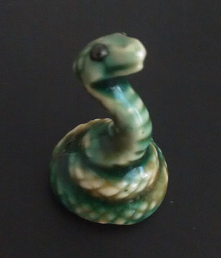
\includegraphics[scale=1]{ular-png}  
	\caption[Gambar {\it Serpentes} dalam format png]{Gambar {\it Serpentes} dalam format png} 
	\label{fig:ularpng} 
\end{figure} 

\dtext{19-20}
\begin{figure}[H]
	\centering  
	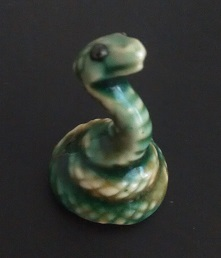
\includegraphics[scale=0.5]{ular-jpg}  
	\caption[Ular kecil]{Ular kecil} 
	\label{fig:ularjpg} 
\end{figure} 
\dtext{21-22}

\begin{figure}[ht] 
	\centering  
	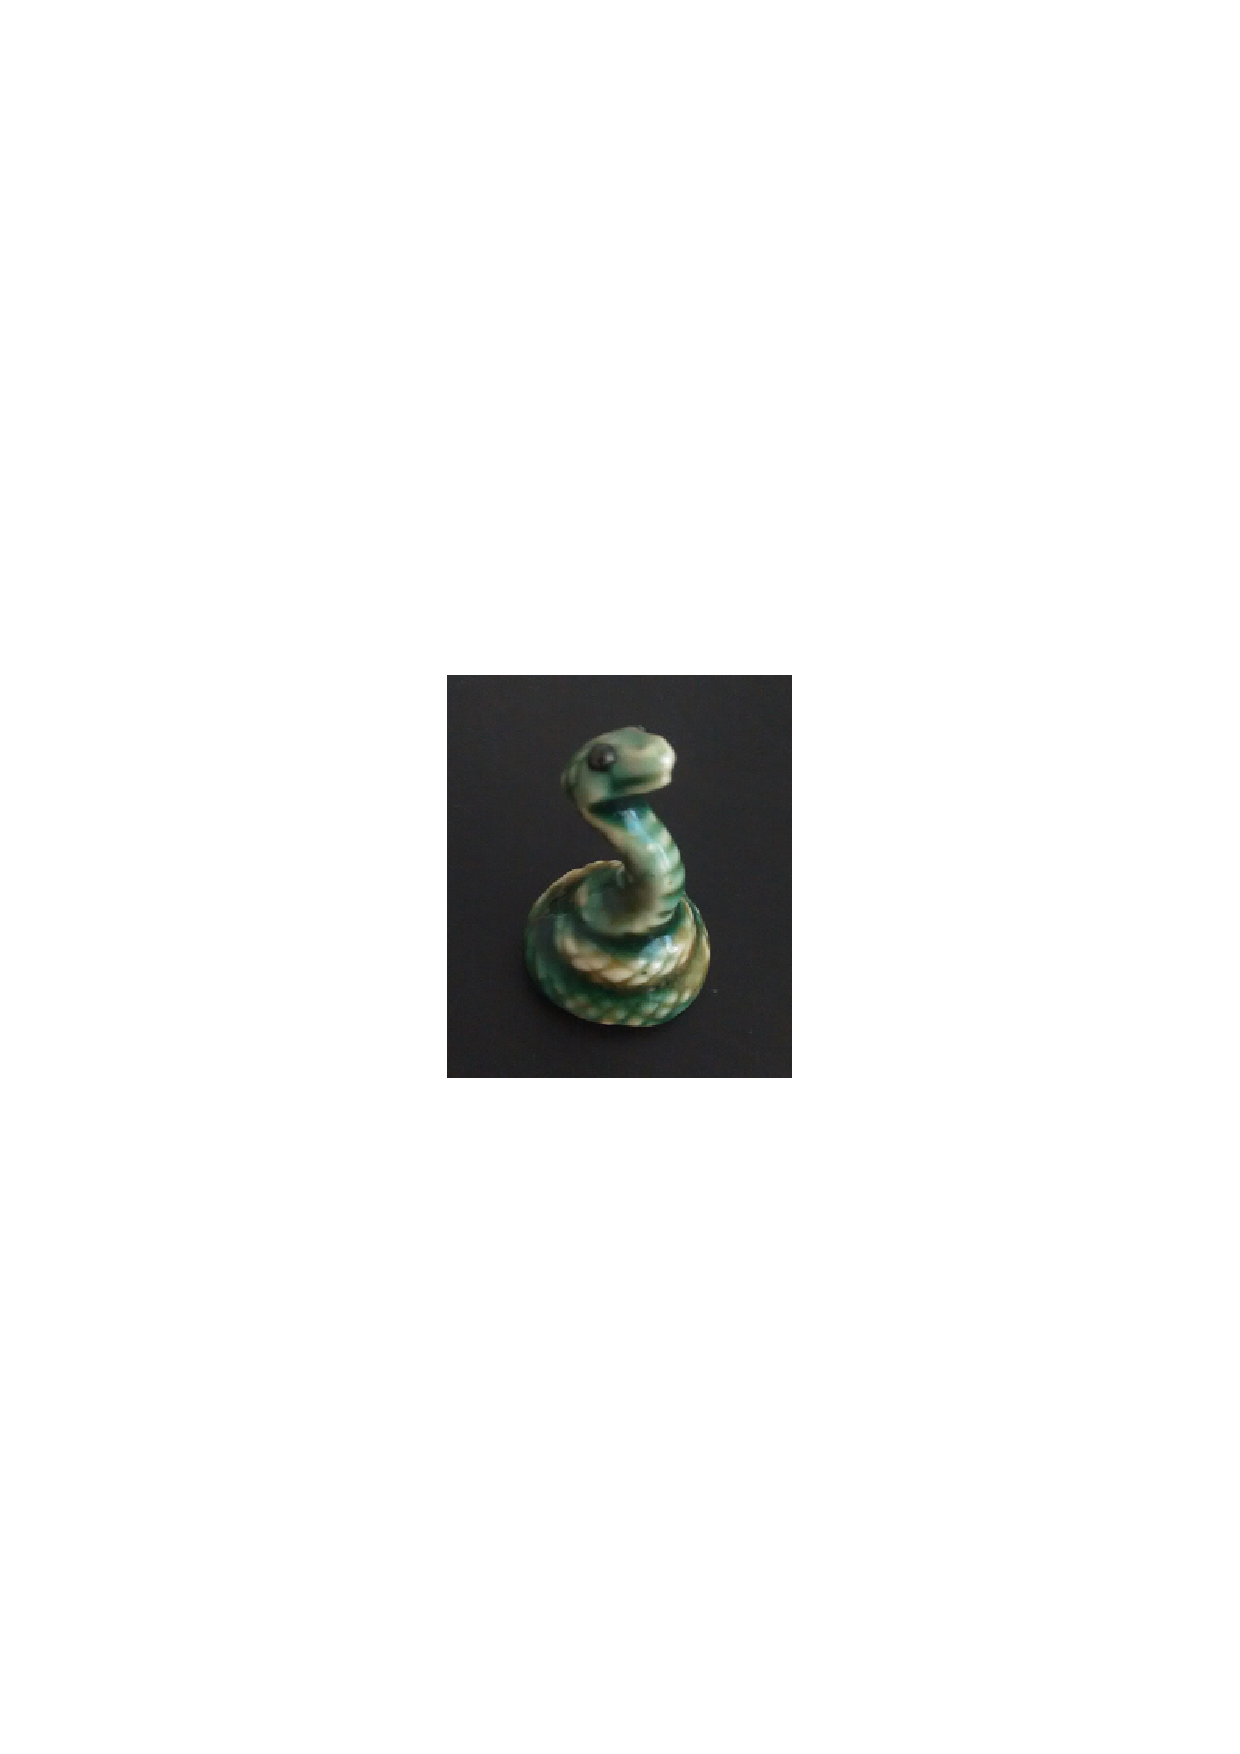
\includegraphics[scale=1]{ular-pdf}  
	\caption[ {\it Serpentes} betina]{ {\it Serpentes} jantan} 
	\label{fig:ularpdf} 
\end{figure} 
 
